\documentclass{article}
\usepackage{bigstrut}
\usepackage{adjustbox}
\usepackage{graphicx}^^M
\graphicspath{ {images/} }
\usepackage[T1]{fontenc}
\usepackage{float}

\usepackage[english]{babel}
\usepackage[utf8]{inputenc}
\usepackage{indentfirst}

\addtolength{\oddsidemargin}{-.875in}
\addtolength{\evensidemargin}{-.875in}
\addtolength{\textwidth}{1.75in}
\addtolength{\textheight}{1in}

\begin{document}
\title{Design V: Lab 6}
\begin{titlepage}
    \centering
	{\scshape\LARGE Lab 6: Dye-Sensitized Solar Cells\par}
	\vspace{1cm}
	{\scshape Alex Smith: Recorder \hfill ID\#:10416940 \par}
	{\scshape Marcin Wisniowski: Manager \hfill ID\#:10417225\par}
	{\scshape Naomi Henderson: Technician \hfill ID\#:10406469\par}
    \vfill
	{\scshape Design V, Week 7\par}
	\vspace{.5cm}
	{\scshape Laboratory Performed: March 6th, 2018\\Stevens Institute of Technology\\E-231 Section I Group 1\par}
	\vspace{.5cm}
	{\scshape supervised by\\Mr. Di Wu, Mr. Kai Zong \par}
    \vfill
% Bottom of the page
	{\scshape“I pledge my honor that I have abided by the Stevens Honor System.”\par}
	\vspace{.5cm}
	{\scshape Alex Smith \hfill Date: 03/19/18\\Marcin Wisniowski \hfill Date: 03/19/18\\ Naomi Henderson \hfill Date: 03/19/18\\}
	\vspace{3cm}
\end{titlepage}

\section{Introduction}
In this lab, the group was tasked to learn about solar energy and the proper steps taken in creating a dye-sensitized solar cell. Solar energy involves capturing and utilizing the energy from sunlight. Since most appliances run on electricity, it is important to transform this sunlight into usage electrical current. This can be achieved by creating solar cells, which generate electrical voltage under light. Furthermore, they can be linked together for more substantial gains in electrical power. While today’s solar cells are made of silicon and are reliable, the manufacturing of these types of cells is expensive and therefore lowers the competitiveness that can be achieved with solar cell pricing. The group looked to observe how using more common and cheaper materials to create a working solar cell for a fraction of the price. In this case, titanium dioxide and a dye extracted from crushed blackberries was used to create the solar cell. 

\subsection{Objectives}
\begin{enumerate}
\item Explore other types of energy production methods that have a less harmful environmental impact.
\item Examine the applications of dye-sensitized solar cells (DSSC) when working with solar energy conversion. 
\item Compare the DSSC to a commercial silicon solar cell to find positive and negative applications of using the DSSC.
\item Compare the output of a DSSC to a cheap Silicon Cell (using light bulb illumination)
\item Learn the steps a typical solar cell goes through to produce electricity and assembly a DSSC cell to work like a typical solar cell.

\end{enumerate}

\subsection{Hypothesis}
The group expects for the DSSC to work far less efficiently than silicon based solar cells due to the less precise conditions of creating it. Similarly, the group expects that the amount of light will have an effect on the voltage and current readings. With less light entering the solar cells, voltage and current will be lower than with more light. Finally, the group believes that a larger active area should provide more voltage and current gain, as there is a larger area that is absorbing the light. 


\section{Procedure}
\subsection{Preparing the Dye Sensitized Electrodes}
The group began by preheating a lab furnace to $450^oC$ for future use. While heating, one slide was prepared for baking. A glass coated with fluorinated tin oxide was cleaned with ethyl alcohol and dried. Then, using scotch tape, three edges of the slide were taped down and covered. White nano-$TiO_2$ was placed within the scotch tape edges and slowly spread for an even coating. A hair dryer was used to speed up the drying process of the $TiO_2$ before removing the tape from the edges and placing the $TiO_2$ covered slide into the furnace.

\subsubsection{Dyeing the Electrodes}
After the sintering process was complete, the glass slide was allowed to cool on a heat resistant tile for 5-10 minutes. In the meantime, two blackberries were crushed with a fork to extract as much juice as possible from them. The liquid was placed through a filter onto a watch glass. Then, the cooled down $TiO_2$ slide was placed face down into the watch glass to dye the area covered by the $TiO_2$. After soaking for 5-10 minutes, the electrode was removed and rinsed several times. Finally, to complete the first slide, the slide was rinsed with ethanol and set on the bench to dry.

\subsubsection{Preparing the Carbon-Coated Counter Electrode}
The other glass slide was picked up and held over a candle flame in order to place a graphitic coating over the surface of the whole electrode. The entire surface was slowly passed through a candle until the surface was entirely black before continuing. 

\subsection{Testing a Silicon Solar Cell}
While waiting for the first glass slide to sinter, a silicon solar cell was tested in order to set a control setting for out experiment to compare to. A multimeter was used to test values along with alligator clips. The silicon cell was placed under a turned-on lamp and the voltage was allowed to reach a stable amount. This was recorded for further reference. Similarly, the multimeter was set to test for current and the values were recorded. Finally, the solar cell was flipped and the lamp was turned off while the cell was still connected to see how the voltage changed after the source of light was removed. This was observed and recorded. Finally, the active area of the silicon solar cell was recorded. 

\subsection{Assembling and Testing the DSSC}
After both electrodes were created, the slide was assembled together. The graphite coated slide was placed on top of the blackberry dyed slide with an offset to allow for alligator clips to latch onto both. Using binder clips the cell was forced together and using iodine solution the cell was stained in order to finish the process of creating the DSSC. Once the DSSC was assembled, it was tested across the same settings as the control silicon solar cell. The positive clip was attached to the graphite covered electrode and the ground electrode to the dyed electrode. The DSSC was placed under a lamp and voltage and current were both observed and recorded. Finally, the active area was measured.


\section{Results}

The power output of the silicon solar cell is: 
$$P = V*I = (4.13 V)(0.0035 A) = 0.014455 W $$

The power output of the DSSC is: 
$$P = V * I = (0.19 V)(22.5 x 10^{-6} A) = 4.275 x 10^{-6} W $$

Normalizing the area, the powers per square millimeter are:
$$Silicon: \frac{0.014455 W}{2350 mm^2} = \frac{6.15 x 10^{-6} W}{mm^2}$$
$$DSSC: \frac{4.275 x 10^{-6} W}{241.37 mm^2} = \frac{1.771  10^{-8} W}{mm^2}$$

This means that to power a 100 W light bulb, these areas would be needed for each source.
$$Silicon: \frac{100 W}{6.15 x 10^{-6} W}{mm^2} = 1.626 x 10^7 mm^2 = 16.26 m^2 $$
$$DSSC: \frac{100 W}{1.771 x 10^{-8} W}{mm^2} = 5.647 x 10^9 mm^2 = 5646 m^2 $$

\begin{figure}
\begin{center}
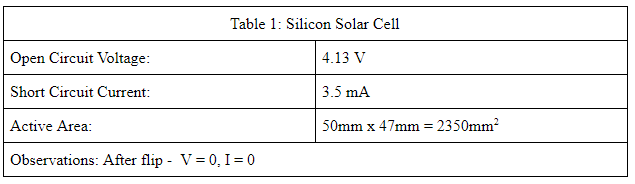
\includegraphics[width=400pt]{Screenshot_1.png}
\caption{Silicon Solar Cell}
\end{center}
\end{figure}

\begin{figure}
\begin{center}
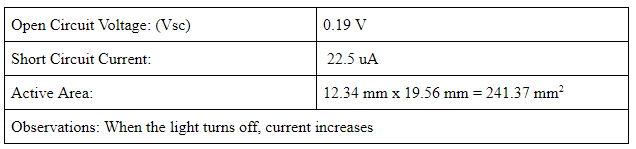
\includegraphics[width=400pt]{Screenshot_2.png}
\caption{Dye-Sensitized Solar Cell}
\end{center}
\end{figure}

\section{Discussion}
Upon completing this experiment, the group found that the silicon based solar cell outperformed the DSSC on a number of different parameters. After normalizing the area for each cell, the silicon solar cell had a greater insulation value at $\frac{6.15E-6 W}{mm^2}$ than that of the DSSC cell at $\frac{1.771E-8 W}{mm^2}$. This was not shocking to the group, as we had already assumed the silicon solar cell would be more efficient than the DSSC. It is also important to note that real-world manufactured DSSC’s have an efficiency of 5\% - 13\% while silicon cells have an efficiency of around 20\% making these real-world DSSC’s efficiency closer to that of silicon cells. The required active area to power a 100W light bulb for a silicon cell would be $16.26 m^2$ while the DSSC would require an area of $5646 m^2$. To put that into perspective, $16.26 m^2$ is about the average size of a one-car garage while $5646 m^2$ is approximately $295 m^2$ larger than an American football field. After the lamp was turned off, the group observed that the silicon based solar cell stopped harnessing power, and its voltage went to zero as well as its current. For the DSSC, however, the current continued to increase after the lamp was turned off, indicating that the cell was still harboring power. This could be due to the fact that the DCCS is more highly sensitive to light, thus, it was able to harness the ambient room lighting once the lamp was turned off. With this observation, the group concluded that the electrons in the silicon cell require a greater amount of energy to force them across the semiconductor than that of the DSSC. the DSSC electrons are more easily excited because they require much less activation energy and they can travel freely through the iodine solution.

The commercially manufactured silicon solar cell is much more efficient than the lab made DSSC at harnessing power, which proves the teams hypothesis about the silicon cell being more efficient than the DSSC. The second hypothesis of the group was that a larger active area for the cell would correlate to a higher voltage and current reading. This was proved by exposing only half of the silicon solar cell to the light and observing the voltmeter. Covering the cell resulted in a drop in both the voltage and current. 



\section{Broader Impacts}
\begin{enumerate}
\item The dye-sensitized solar cell by absorbing light from the sun to generate a voltage. The cells the team made in class had relatively flat surfaces and were covered with dye within a specific surface area. In the manual illustration, another kind of cell has a notched surface instead of a continuous plane. This design would make a more effective cell because there would be much more surface area exposed to light. This means more sunlight could be processed and thus, the cell would be more powerful.

\item 
\begin{itemize}
\item Given the United States power requirement of $0.46*10^{12}$ Watts at any time, and the average solar power incidence as $7 Watts/ft^2$, the following stands:
		$$(0.46 * 10^{12} W)(\frac{1 ft^2}{7 W}) = 6.57*10^{10} ft^2$$

Since a DSSC can only output 10\% of its absorbed power, that value needs to be multiplied by 10. Converting to more useful units gives 23,570 square miles, which is approximately equal to the area of West Virginia, which is 24,077 square miles.

\item Given the New York Times ability to print on 4 foot wide paper at a rate of 3000 feet/second, they can print 12000 square feet / second. Knowing that gives this equation: 
$$(6.57*10^{11} ft^2)(\frac{1 second}{12000 ft^2})(\frac{1 year}{3600 seconds}) = 15,208 years$$ 
It will take 15,208 years for the New York Times to print enough DSSCs to support the United States.
\end{itemize}
\end{enumerate}

\end{document}